\chapter{Reproducción sexual de las plantas con flores}\label{ch:b2:angiosperm-reproduction}

Un manzanar en mayo está blanco de \omterm{def:b2:angiosperm-reproduction:flower}{flores} y lleno del zumbido de las
abejas; en octubre los mismos árboles están cargados de fruta, cada
manzana con diez \omterm{def:b2:angiosperm-reproduction:seed}{semillas}, cada \omterm{def:b2:angiosperm-reproduction:seed}{semilla} un árbol embrionario envuelto en
una reserva de alimento. Toda esa transformación --- la \omterm{def:b2:angiosperm-reproduction:flower}{flor}, el \omterm{def:b2:plant-life-cycles:heterospory}{polen}
transportado por un insecto, el tubo que crece a través del estilo, la
\omterm{prop:b2:angiosperm-reproduction:double}{doble fecundación} que produce a la vez un embrión y su provisión de
alimento, el \omterm{def:b2:angiosperm-reproduction:flower}{ovario} que se hincha hasta convertirse en un \omterm{def:b2:angiosperm-reproduction:seed}{fruto} hecho
para ser comido --- es la invención que convirtió a las plantas con
\omterm{def:b2:angiosperm-reproduction:flower}{flores}, en cien millones de años, en las plantas \omterm{def:b2:meiosis-heredity:vocabulary}{dominantes} de la
tierra firme. Este capítulo la sigue desde la \omterm{def:b2:angiosperm-reproduction:flower}{flor} hasta la \omterm{def:b2:angiosperm-reproduction:seed}{semilla}
dispersada.

\section{La flor}

\begin{definition}[Las partes de una flor]\label{def:b2:angiosperm-reproduction:flower}
\index{flor}\index{estambre}\index{carpelo}\index{ovario}\index{estigma}
Una \emph{flor} es un tallo corto cuyas hojas se han transformado en
cuatro verticilos. Por fuera, los \emph{sépalos} (en conjunto, el cáliz)
protegen el botón; después, los \emph{pétalos} (la corola), que atraen;
después, los \emph{estambres}, cada uno un filamento que lleva una
\emph{antera} con cuatro sacos polínicos; y en el centro uno o varios
\emph{carpelos}, cada uno plegado y soldado en un \emph{pistilo} con un
\emph{estigma} receptivo, un \emph{estilo} y un \emph{ovario} que
encierra los \emph{óvulos}. Una flor con estambres y carpelos a la vez es
\emph{hermafrodita} (la mayoría de las especies); las plantas
\emph{monoicas} llevan flores masculinas y femeninas separadas en un
mismo individuo (maíz, roble, avellano), y las especies \emph{dioicas},
en individuos distintos (acebo, sauce, palmera datilera). Toda la razón
de ser del carpelo cerrado --- el carácter que da nombre a las
angiospermas --- es que los óvulos quedan encerrados: el \omterm{def:b2:plant-life-cycles:heterospory}{polen} nunca los
alcanza directamente, sino que debe crecer hasta ellos a través del
tejido de la planta, lo que permite a la planta elegir.
\end{definition}

\begin{omfigure}
\begin{tikzpicture}[every node/.style={font=\scriptsize}]
  % receptacle and pedicel
  \draw[thick] (0,-2.6) -- (0,-1.6);
  \draw[thick, fill=omExo!20] (-0.9,-1.6) .. controls (-1.0,-1.0) and (1.0,-1.0) .. (0.9,-1.6) -- cycle;
  % sepals
  \foreach \s in {-1,1} \draw[thick, fill=omExo!45] (0.6*\s,-1.4) .. controls (2.0*\s,-1.2) and (2.6*\s,-0.2) .. (2.8*\s,0.6) .. controls (2.0*\s,0.2) and (1.2*\s,-0.6) .. (0.6*\s,-1.4);
  % petals
  \foreach \s in {-1,1} \draw[thick, fill=omThm!15] (0.5*\s,-1.2) .. controls (1.6*\s,0.4) and (2.2*\s,1.8) .. (1.6*\s,3.0) .. controls (1.0*\s,2.0) and (0.5*\s,0.8) .. (0.5*\s,-1.2);
  % ovary with ovules
  \draw[thick, fill=omDef!12] (0,-0.7) ellipse (0.55 and 0.75);
  \foreach \p in {(-0.22,-0.5),(-0.22,-0.9),(0.22,-0.5),(0.22,-0.9)} \draw[thick, omDef, fill=omDef!40] \p circle (0.11);
  % style and stigma
  \draw[thick, fill=omDef!12] (-0.1,0.05) rectangle (0.1,1.9);
  \draw[thick, fill=omDef!40] (0,2.0) ellipse (0.28 and 0.14);
  % stamens
  \foreach \s in {-1,1} { \draw[thick] (0.35*\s,-1.0) .. controls (0.6*\s,0.2) .. (0.9*\s,1.5); \draw[thick, fill=omProp!60] (0.9*\s,1.6) ellipse (0.14 and 0.32); }
  % labels: right side
  \draw (0.28,2.0) -- (3.2,2.6) node[right] {estigma};
  \draw (0.1,1.2) -- (3.2,1.9) node[right] {estilo};
  \draw (0.55,-0.6) -- (3.2,1.2) node[right] {ovario};
  \draw (0.22,-0.9) -- (3.2,0.5) node[right] {óvulo};
  \draw (2.6,0.35) -- (3.2,-0.4) node[right] {sépalo};
  % labels: left side
  \draw (-1.5,2.4) -- (-2.6,2.8) node[left] {pétalo};
  \draw (-0.95,1.9) -- (-2.6,1.9) node[left] {antera};
  \draw (-0.65,0.6) -- (-2.6,0.9) node[left] {filamento};
  \draw (0,-2.2) -- (-2.6,-2.2) node[left] {receptáculo y pedúnculo};
  \node[anchor=west, align=left] at (5.4,0.5) {estigma + estilo + ovario\\$=$ el carpelo (pistilo)};
  \node[anchor=west, align=left] at (5.4,-0.8) {antera + filamento\\$=$ el estambre};
\end{tikzpicture}

{\small Una \omterm{def:b2:angiosperm-reproduction:flower}{flor} en sección longitudinal: sépalos, pétalos, \omterm{def:b2:angiosperm-reproduction:flower}{estambres}
(filamento y antera) y, en el centro, el \omterm{def:b2:angiosperm-reproduction:flower}{carpelo} --- \omterm{def:b2:angiosperm-reproduction:flower}{estigma}, estilo y
\omterm{def:b2:angiosperm-reproduction:flower}{ovario} --- que encierra los óvulos.}
\end{omfigure}

\begin{omfigure}
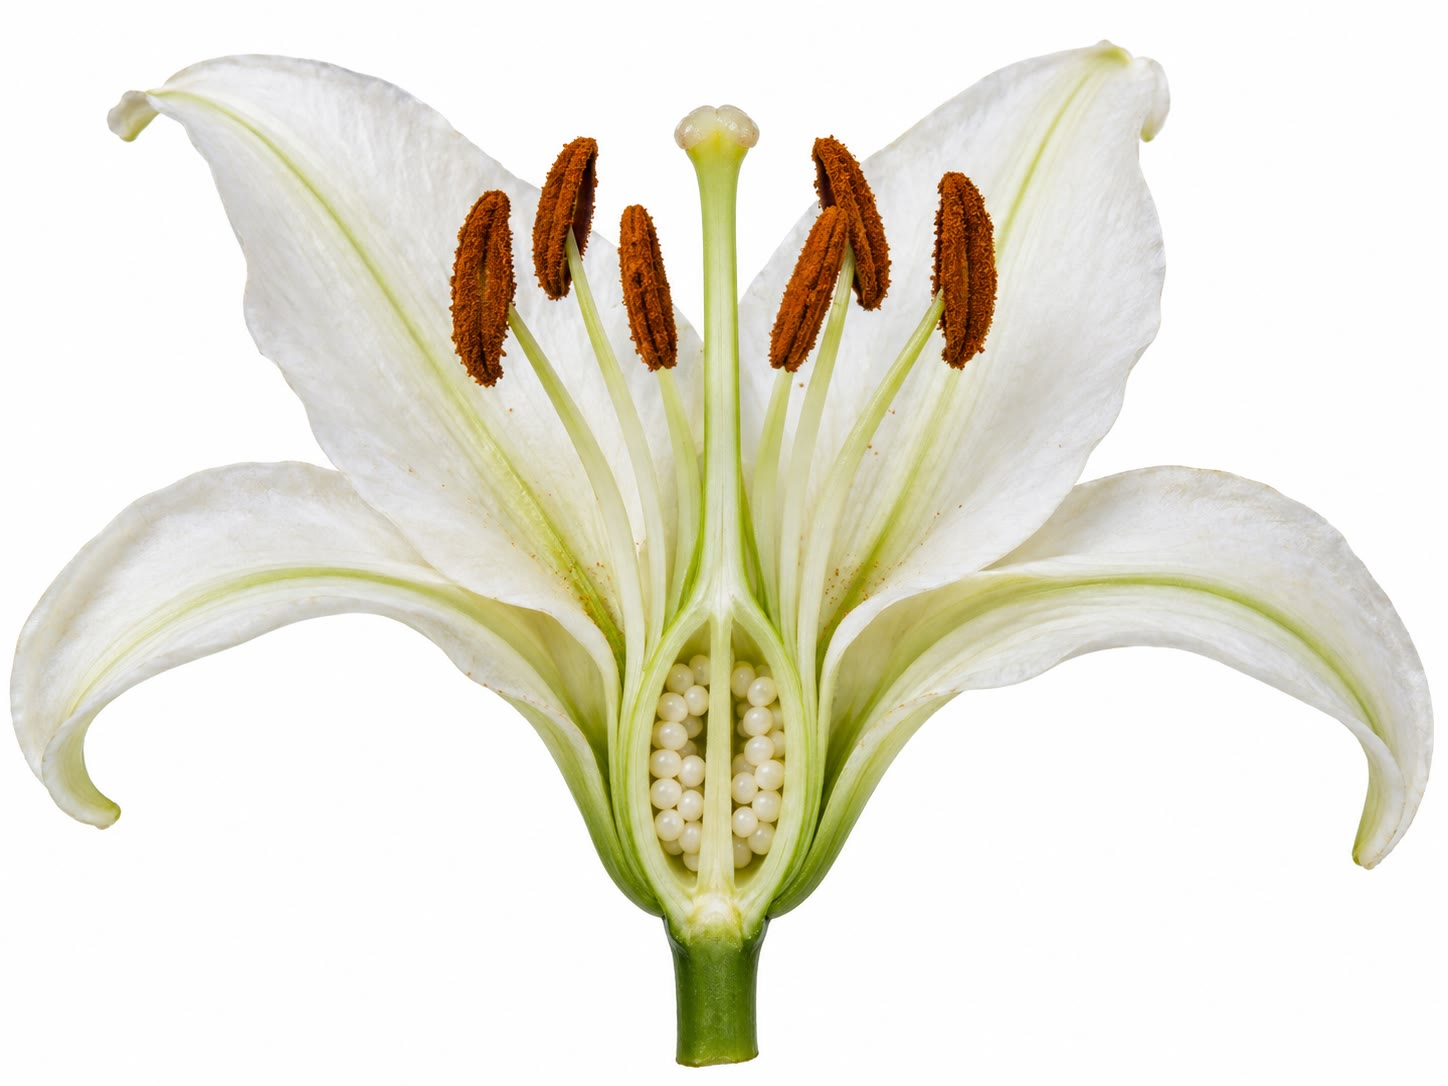
\includegraphics[width=0.55\linewidth]{images/book4/ai/b4-06-lily-dissected.jpg}

{\small Un lirio cortado a lo largo: seis \omterm{def:b2:angiosperm-reproduction:flower}{estambres} con las anteras
cargadas de \omterm{def:b2:plant-life-cycles:heterospory}{polen}, el largo estilo con su \omterm{def:b2:angiosperm-reproduction:flower}{estigma} pegajoso y el \omterm{def:b2:angiosperm-reproduction:flower}{ovario}
abierto para mostrar las hileras de óvulos.}
\end{omfigure}

\section{Los dos gametofitos}

\begin{proposition}[El polen: el gametofito masculino]\label{prop:b2:angiosperm-reproduction:pollen}
\index{grano de polen}\index{microsporogénesis}\index{esporopolenina}
En cada saco polínico, células madre \omterm{def:b2:meiosis-heredity:meiosis}{diploides} sufren la \omterm{def:b2:meiosis-heredity:meiosis}{meiosis} y dan
tétradas de \emph{\omterm{def:b2:plant-life-cycles:heterospory}{microsporas}}. Cada \omterm{def:b2:plant-life-cycles:heterospory}{microspora} se divide una vez, de
forma desigual, en una gran \emph{célula vegetativa} y una pequeña
\emph{célula generativa} englobada en ella; la célula generativa se
divide una vez más, antes o después de la \omterm{def:b2:angiosperm-reproduction:pollination}{polinización}, en dos
\emph{células espermáticas}. El \emph{\omterm{prop:b2:angiosperm-reproduction:pollen}{grano de polen}} maduro es, pues, un
organismo \omterm{def:b2:meiosis-heredity:meiosis}{haploide} de tres células --- todo el \omterm{def:b2:plant-life-cycles:cycles}{gametofito} masculino ---
de \qtyrange{10}{100}{\micro m}, sellado en una pared cuya capa externa de
\emph{esporopolenina}, el polímero biológico más resistente que se
conoce, está esculpida con espinas, poros y surcos característicos de
cada especie, y por eso el \omterm{def:b2:plant-life-cycles:heterospory}{polen} permite identificar plantas en
sedimentos de decenas de millones de años. El grano se libera
deshidratado y sobrevive de horas (gramíneas) a semanas (algunos
árboles) hasta llegar a un \omterm{def:b2:angiosperm-reproduction:flower}{estigma}.
\end{proposition}

\begin{omfigure}
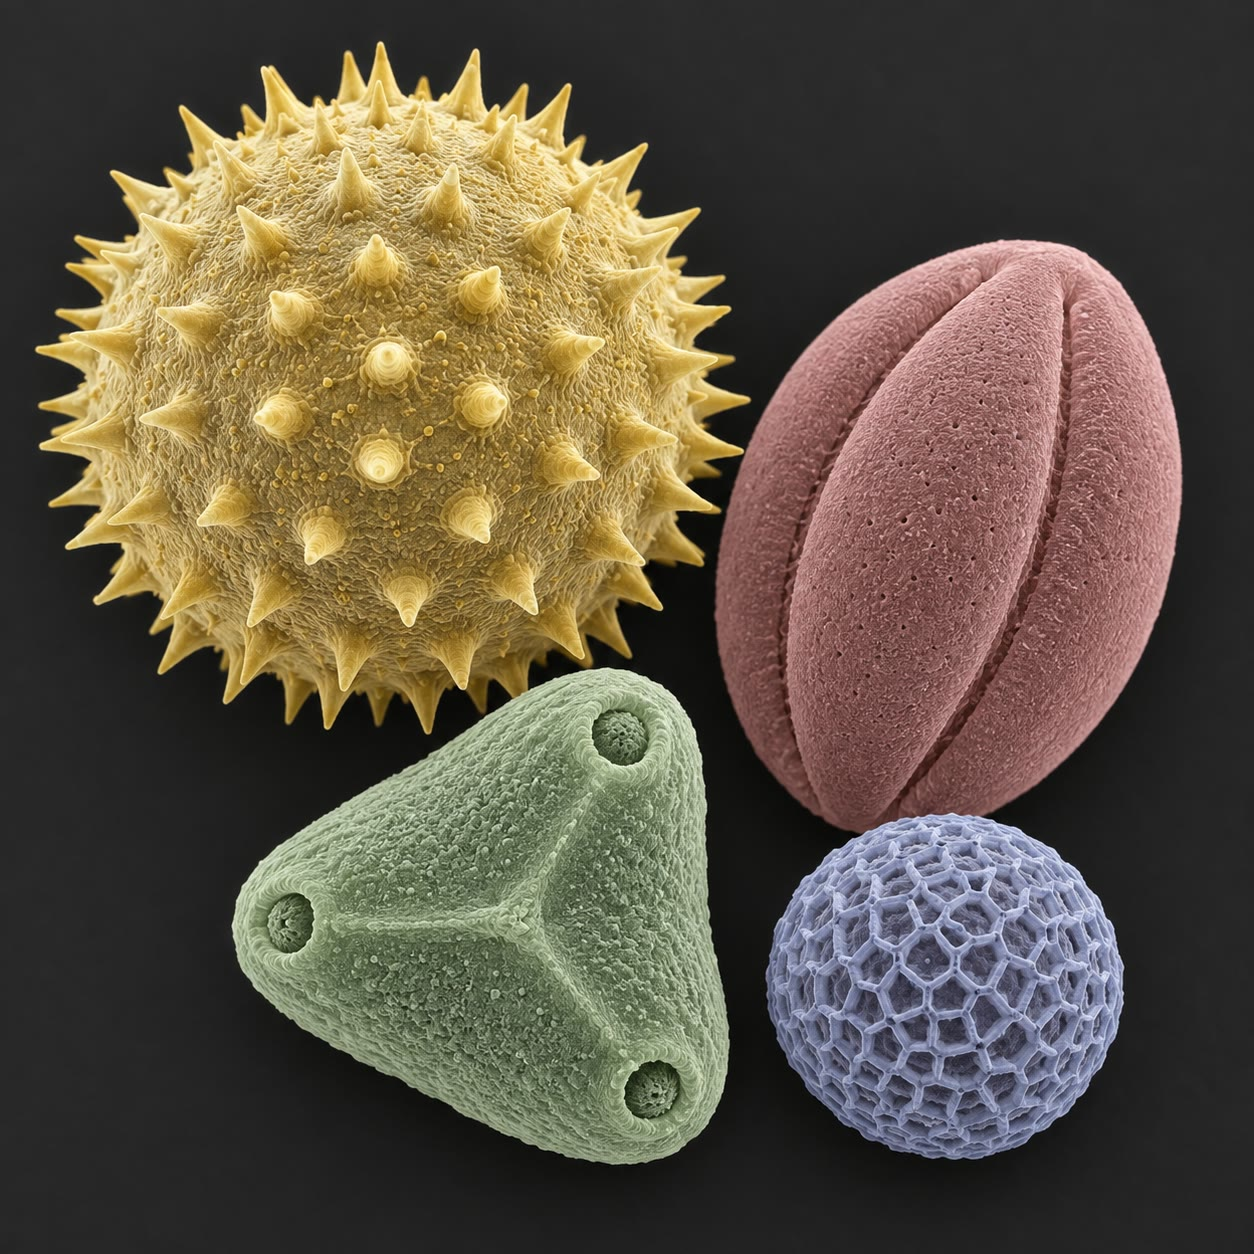
\includegraphics[width=0.45\linewidth]{images/book4/ai/b4-06-pollen-sem.jpg}

{\small \omterm{prop:b2:angiosperm-reproduction:pollen}{Granos de polen} al microscopio electrónico de barrido: la pared
de esporopolenina de cada especie tiene su propia escultura ---
espinas, surcos, poros, un retículo --- por la que puede reconocerse.}
\end{omfigure}

\begin{proposition}[El saco embrionario: el gametofito femenino]\label{prop:b2:angiosperm-reproduction:embryosac}
\index{saco embrionario}\index{megasporogénesis}\index{núcleos polares}
En cada óvulo, una célula \omterm{def:b2:meiosis-heredity:meiosis}{diploide} de la nucela sufre la \omterm{def:b2:meiosis-heredity:meiosis}{meiosis}; tres
de las cuatro \omterm{def:b2:plant-life-cycles:heterospory}{megasporas} degeneran y la cuarta da, mediante tres mitosis
sin división celular, un \emph{\omterm{prop:b2:angiosperm-reproduction:embryosac}{saco embrionario}} de ocho núcleos y siete
células: en el extremo micropilar, la \emph{oosfera}
flanqueada por dos \emph{sinérgidas}; en el extremo opuesto, tres células
\emph{antípodas}; en el centro, una gran \emph{célula central} que
contiene dos \emph{\omterm{prop:b2:angiosperm-reproduction:embryosac}{núcleos polares}}. Este saco, envuelto en la nucela y
en dos tegumentos con un micrópilo, es todo el \omterm{def:b2:plant-life-cycles:cycles}{gametofito} femenino ---
siete células donde un \omterm{def:b2:plant-life-cycles:moss}{musgo} tenía una planta. Los dos \omterm{prop:b2:angiosperm-reproduction:embryosac}{núcleos polares}
son genéticamente idénticos a la oosfera, un hecho que importa para el
endospermo.
\end{proposition}

\begin{omfigure}
\begin{tikzpicture}[every node/.style={font=\scriptsize}]
  % pollen grain
  \begin{scope}
    \draw[very thick, omProp!80!black, fill=omProp!15] (0,0) circle (1.1);
    \draw[thick, omProp!80!black] (0,0) circle (0.95);
    \foreach \a in {0,30,...,330} \draw[omProp!80!black, thick] (\a:1.1) -- (\a:1.25);
    \draw[thick, fill=omDef!25] (0.15,-0.2) ellipse (0.55 and 0.4); \node[font=\tiny] at (0.15,-0.2) {vegetativa};
    \draw[thick, fill=omThm!30] (-0.3,0.45) ellipse (0.22 and 0.14); \draw[thick, fill=omThm!30] (0.2,0.5) ellipse (0.22 and 0.14);
    \draw[omThm] (0.0,0.62) -- (0.0,1.5); \node[omThm, anchor=south] at (0.0,1.5) {dos células espermáticas};
    \node[below, align=center] at (0,-1.4) {grano de polen ($n$)\\3 células, pared de esporopolenina};
  \end{scope}
  % ovule with embryo sac
  \begin{scope}[xshift=5.5cm]
    \draw[thick, fill=omExo!25] (0,0) ellipse (1.5 and 2.1);
    \draw[thick, fill=omExo!10] (0,0) ellipse (1.15 and 1.75);
    \fill[white] (-0.3,1.7) rectangle (0.3,2.2); \draw[thick] (-0.3,1.7) -- (-0.3,2.15); \draw[thick] (0.3,1.7) -- (0.3,2.15);
    \draw[thick, fill=white] (0,0) ellipse (0.7 and 1.35);
    % cells: egg + synergids top, central, antipodals bottom
    \draw[thick, fill=omThm!30] (0,0.95) circle (0.17); \node[omThm, anchor=west] at (1.6,1.2) {oosfera};
    \draw[thick, fill=omDef!25] (-0.35,1.0) circle (0.14); \draw[thick, fill=omDef!25] (0.35,1.0) circle (0.14); \node[anchor=west] at (1.6,0.75) {dos sinérgidas};
    \draw[thick, fill=omDef!10] (0,0) ellipse (0.55 and 0.6); \fill[omDef!80!black] (-0.15,0.05) circle (0.09); \fill[omDef!80!black] (0.15,0.05) circle (0.09);
    \node[anchor=west, align=left] at (1.6,0.1) {célula central con\\dos núcleos polares};
    \foreach \x in {-0.3,0,0.3} \draw[thick, fill=omDef!25] (\x,-1.0) circle (0.13); \node[anchor=west] at (1.6,-1.0) {tres antípodas};
    \draw (0.35,2.0) -- (1.6,2.0) node[right] {micrópilo};
    \draw (1.3,-0.9) -- (1.6,-1.6) node[right] {tegumentos};
    \draw (0.9,-1.35) -- (1.6,-2.1) node[right] {nucela};
    \draw (1.6,1.2) -- (0.17,0.95); \draw (1.6,0.75) -- (0.49,1.0); \draw (1.6,0.1) -- (0.55,0.05); \draw (1.6,-1.0) -- (0.43,-1.0);
    \node[below, align=center] at (0,-2.3) {óvulo con saco embrionario ($n$)\\7 células, 8 núcleos};
  \end{scope}
\end{tikzpicture}

{\small Los dos \omterm{def:b2:plant-life-cycles:cycles}{gametofitos} de una planta con \omterm{def:b2:angiosperm-reproduction:flower}{flores}, ambos reducidos a
unas pocas células: el \omterm{prop:b2:angiosperm-reproduction:pollen}{grano de polen} de tres células y el \omterm{prop:b2:angiosperm-reproduction:embryosac}{saco
embrionario} de siete células dentro del óvulo.}
\end{omfigure}

\section{La polinización}

\begin{definition}[La polinización y sus agentes]\label{def:b2:angiosperm-reproduction:pollination}
\index{polinización}\index{síndrome de polinización}\index{néctar}
La \emph{polinización} es la transferencia del \omterm{def:b2:plant-life-cycles:heterospory}{polen} de una antera a un
\omterm{def:b2:angiosperm-reproduction:flower}{estigma}: \emph{autopolinización} dentro de una misma \omterm{def:b2:angiosperm-reproduction:flower}{flor} o planta,
\emph{polinización cruzada} entre plantas distintas. Las \omterm{def:b2:angiosperm-reproduction:flower}{flores}
\emph{anemófilas} (gramíneas, robles, abedules, llantenes) son pequeñas,
verdes, sin olor, con grandes \omterm{def:b2:angiosperm-reproduction:flower}{estigmas} plumosos y cantidades enormes de
\omterm{def:b2:plant-life-cycles:heterospory}{polen} liso y seco; su relación \omterm{def:b2:plant-life-cycles:heterospory}{polen}/óvulo llega al millón. Las \omterm{def:b2:angiosperm-reproduction:flower}{flores}
\emph{zoófilas} pagan a su transportista: \emph{néctar} (una solución
azucarada de los nectarios), el propio \omterm{def:b2:plant-life-cycles:heterospory}{polen}, aceites, perfume; y se
anuncian con un color, una forma y un olor ajustados a los sentidos del
transportista --- guías de néctar ultravioletas para las abejas, que ven
el ultravioleta y no el rojo; \omterm{def:b2:angiosperm-reproduction:flower}{flores} rojas tubulares sin olor para los
colibríes; \omterm{def:b2:angiosperm-reproduction:flower}{flores} blancas, muy perfumadas, de apertura nocturna y tubo
profundo para las polillas; \omterm{def:b2:angiosperm-reproduction:flower}{flores} pardas y fétidas para las moscas de
la carroña; \omterm{def:b2:angiosperm-reproduction:flower}{flores} nocturnas robustas y pálidas para los murciélagos.
Cada uno de estos conjuntos de rasgos es un \emph{síndrome de
polinización}, y el ajuste entre \omterm{def:b2:angiosperm-reproduction:flower}{flor} y polinizador es el caso de manual
de la \emph{coevolución}: Darwin predijo, a partir del espolón nectarífero
de \qty{30}{cm} de una orquídea de Madagascar, una polilla con una
lengua de \qty{30}{cm}, que se encontró cuarenta años después.
\end{definition}

\begin{omfigure}
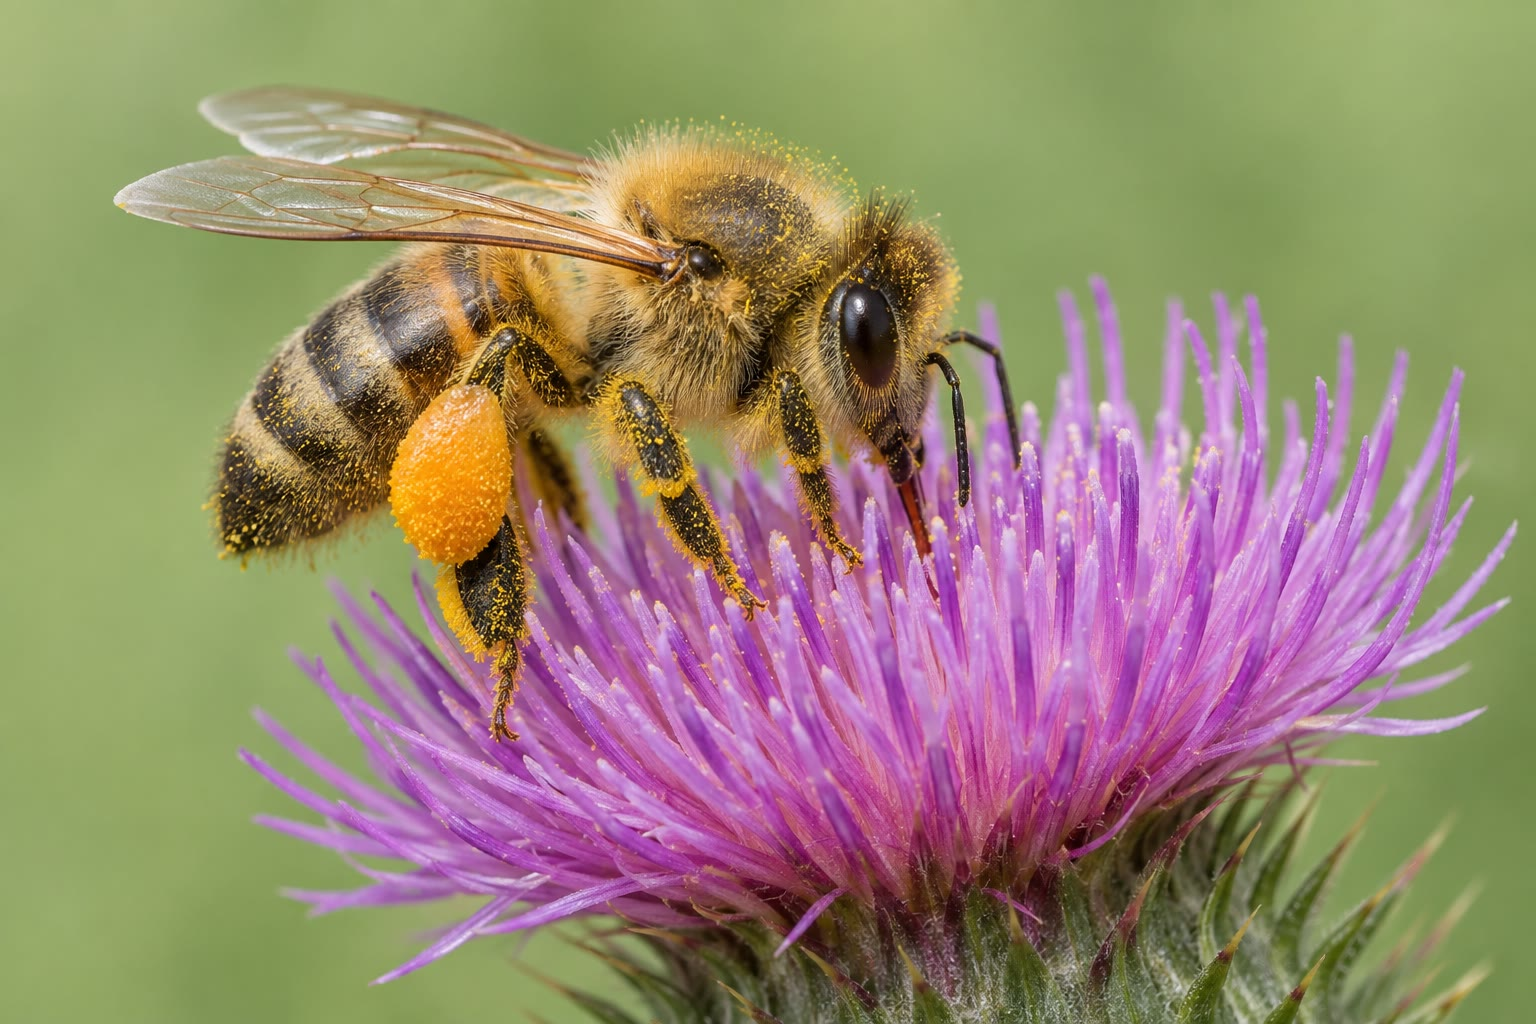
\includegraphics[width=0.58\linewidth]{images/book4/ai/b4-06-bee-on-flower.jpg}

{\small Una abeja melífera sobre un cardo: el \omterm{def:b2:plant-life-cycles:heterospory}{polen} le empolva el cuerpo
y llena las cestillas de sus patas traseras; parte de él llegará al
\omterm{def:b2:angiosperm-reproduction:flower}{estigma} del siguiente cardo que visite. El color púrpura, una plataforma
de aterrizaje y un \omterm{def:b2:angiosperm-reproduction:pollination}{néctar} abundante constituyen el síndrome de las
abejas.}
\end{omfigure}

\begin{proposition}[Evitar la autofecundación]\label{prop:b2:angiosperm-reproduction:selfing}
\index{autoincompatibilidad}\index{heterostilia}\index{dicogamia}
Una \omterm{def:b2:angiosperm-reproduction:flower}{flor} hermafrodita podría fecundarse a sí misma, y muchas lo hacen
(guisantes, trigo, tomates); pero la autofecundación deja al descubierto
los \omterm{def:b2:meiosis-heredity:vocabulary}{alelos} \omterm{def:b2:meiosis-heredity:vocabulary}{recesivos} perjudiciales (\emph{depresión por endogamia}), y la
mayoría de las especies la impide. En el tiempo: \emph{dicogamia},
anteras y \omterm{def:b2:angiosperm-reproduction:flower}{estigma} que maduran en momentos distintos (protandria en la
mayoría de las umbelíferas y compuestas). En el espacio:
\emph{hercogamia}, anteras y \omterm{def:b2:angiosperm-reproduction:flower}{estigma} separados, como en la
\emph{heterostilia} de las prímulas, cuyas \omterm{def:b2:angiosperm-reproduction:flower}{flores} longistilas (estilo
largo, anteras bajas) y brevistilas (estilo corto, anteras altas)
depositan el \omterm{def:b2:plant-life-cycles:heterospory}{polen} en partes distintas del insecto. Bioquímicamente:
\emph{autoincompatibilidad}, un sistema de reconocimiento en el que se
rechaza el \omterm{def:b2:plant-life-cycles:heterospory}{polen} que lleva un \omterm{def:b2:meiosis-heredity:vocabulary}{alelo} $S$ compartido con el pistilo. En la
incompatibilidad \emph{gametofítica} (manzanos, cerezos, petunias,
gramíneas) decide el propio \omterm{def:b2:meiosis-heredity:vocabulary}{alelo} $S$ \omterm{def:b2:meiosis-heredity:meiosis}{haploide} del \omterm{def:b2:plant-life-cycles:heterospory}{polen}: un pistilo
$S_1S_2$ detiene en el estilo los tubos $S_1$ y $S_2$, de modo que el
\omterm{def:b2:plant-life-cycles:heterospory}{polen} de una planta $S_1S_3$ es compatible a medias y el de una $S_3S_4$,
por completo. En la incompatibilidad \emph{esporofítica} (coles,
girasoles) decide el \omterm{def:b2:meiosis-heredity:vocabulary}{genotipo} \omterm{def:b2:meiosis-heredity:meiosis}{diploide} de la planta que produjo el \omterm{def:b2:plant-life-cycles:heterospory}{polen},
en la superficie del \omterm{def:b2:angiosperm-reproduction:flower}{estigma}. Un \omterm{def:b2:meiosis-heredity:vocabulary}{alelo} $S$ raro es compatible con casi
todas las parejas, de modo que la selección mantiene decenas de \omterm{def:b2:meiosis-heredity:vocabulary}{alelos}
en una población.
\end{proposition}
\begin{proof}[Evidencia]
Darwin (1862, 1877) cruzó prímulas a mano: el \omterm{def:b2:plant-life-cycles:heterospory}{polen} de una \omterm{def:b2:angiosperm-reproduction:flower}{flor}
brevistila sobre un \omterm{def:b2:angiosperm-reproduction:flower}{estigma} longistilo (una unión ``legítima'') daba
cápsulas llenas; longistila sobre longistila o brevistila sobre
brevistila (``ilegítimas'') daban pocas \omterm{def:b2:angiosperm-reproduction:seed}{semillas} o ninguna, aunque las
plantas estaban sanas y el \omterm{def:b2:plant-life-cycles:heterospory}{polen} vivo. Concluyó que las dos formas
estaban mutuamente adaptadas al cruzamiento y protegidas de la
autofecundación y, contando las \omterm{def:b2:angiosperm-reproduction:seed}{semillas} por cápsula en miles de
cruzamientos, midió el coste de la autofecundación en decenas de
especies: los descendientes autofecundados eran más bajos, más ligeros y
menos fértiles, generación tras generación.
\end{proof}

\begin{omfigure}
\begin{tikzpicture}[every node/.style={font=\scriptsize}]
  % pistil S1S2 with pollen tubes
  \draw[thick, fill=omDef!10] (-0.5,0) rectangle (0.5,3.2);
  \draw[thick, fill=omDef!30] (0,3.3) ellipse (0.7 and 0.2);
  \draw[thick, fill=omDef!12] (0,-0.6) ellipse (0.9 and 0.7);
  \node at (0,-0.6) {ovario};
  \node[anchor=east] at (-1.1,3.3) {estigma de una planta $S_1S_2$};
  % pollen grains
  \draw[thick, fill=omThm!40] (-0.35,3.75) circle (0.13); \node[omThm, left] at (-0.5,3.75) {$S_1$};
  \draw[thick, fill=omThm!40] (0,3.75) circle (0.13); \node[omThm, anchor=south] at (0,3.92) {$S_2$};
  \draw[thick, fill=omExo!70!black] (0.35,3.75) circle (0.13); \node[right] at (0.5,3.75) {$S_3$};
  % tubes: S1 and S2 stop in the style, S3 reaches the ovary
  \draw[thick, omThm] (-0.35,3.3) -- (-0.35,2.3); \node[omThm, left, align=right] at (-0.55,2.3) {tubo $S_1$\\detenido};
  \draw[thick, omThm] (0,3.3) -- (0,2.0);
  \draw[thick, omExo!70!black] (0.35,3.3) -- (0.35,-0.2) -- (0.2,-0.5);
  \node[right, align=left] at (0.55,0.9) {el tubo $S_3$\\llega a un óvulo};
  \node[anchor=west, align=left, text width=6cm] at (3.2,3.2) {autoincompatibilidad gametofítica: un tubo polínico cuyo propio alelo $S$ coincide con uno de los alelos del pistilo se detiene en el estilo};
  \node[anchor=west, align=left, text width=6cm] at (3.2,1.4) {polen de una planta $S_1S_2$: 0 compatible\\de $S_1S_3$: la mitad\\de $S_3S_4$: todo};
\end{tikzpicture}

{\small Autoincompatibilidad gametofítica. En un pistilo $S_1S_2$, los
tubos que llevan $S_1$ o $S_2$ se detienen en el estilo; un tubo $S_3$
crece hasta el \omterm{def:b2:angiosperm-reproduction:flower}{ovario}.}
\end{omfigure}

\section{La fecundación}

\begin{theorem}[El tubo polínico]\label{thm:b2:angiosperm-reproduction:tube}
\index{tubo polínico}
Un \omterm{prop:b2:angiosperm-reproduction:pollen}{grano de polen} sobre un \omterm{def:b2:angiosperm-reproduction:flower}{estigma} compatible se rehidrata y forma un
\emph{\omterm{thm:b2:angiosperm-reproduction:tube}{tubo polínico}}: la célula vegetativa se alarga por crecimiento
apical, depositando pared nueva en el ápice a razón de
\qtyrange{0.1}{1}{cm/h}, abriéndose paso por digestión a través del
tejido de transmisión del estilo y alimentándose de él. El tubo lleva las
dos células espermáticas en su extremo; unos péptidos secretados por las
sinérgidas lo guían en el último tramo, entra en el óvulo por el
micrópilo, irrumpe en una sinérgida y libera las células espermáticas.
Un tubo que atraviesa un estilo de longitud $L$ a velocidad $v$ tarda
$L/v$: unas pocas horas en un cerezo, un día entero en el maíz, cuyas
``sedas'' son estilos de \qty{20}{cm} de largo. La viabilidad del \omterm{def:b2:plant-life-cycles:heterospory}{polen}
marca un reloj: el \omterm{def:b2:plant-life-cycles:heterospory}{polen} de las gramíneas muere en horas, de modo que
debe alcanzar un \omterm{def:b2:angiosperm-reproduction:flower}{estigma} deprisa.
\end{theorem}
\begin{proof}
El tiempo es la longitud dividida por la velocidad de crecimiento; para el
maíz, \qty{20}{cm} a \qty{1}{cm/h} dan \qty{20}{h}. El propio tubo está
formado casi por completo por pared y una fina película de citoplasma
detrás del ápice, de modo que las reservas de la célula vegetativa, más
lo que absorbe del estilo, bastan para una longitud mil veces mayor que
el diámetro del grano.
\end{proof}

\begin{proposition}[La doble fecundación]\label{prop:b2:angiosperm-reproduction:double}
\index{doble fecundación}\index{endospermo}
De las dos células espermáticas que entrega el tubo, una se fusiona con
la oosfera y forma el \emph{cigoto} \omterm{def:b2:meiosis-heredity:meiosis}{diploide}, del que crece el embrión;
la otra se fusiona con la célula central y sus dos \omterm{prop:b2:angiosperm-reproduction:embryosac}{núcleos polares} y forma
un núcleo \emph{triploide} ($3n$: dos genomas maternos y uno paterno),
del que crece el \emph{endospermo} --- un tejido nutritivo que llena la
\omterm{def:b2:angiosperm-reproduction:seed}{semilla} de almidón, aceite y proteína. Ambas fecundaciones ocurren con
minutos de diferencia; en la mayoría de las especies ninguna prospera
sin la otra, de modo que la planta solo aprovisiona las \omterm{def:b2:angiosperm-reproduction:seed}{semillas} que
llevan un embrión. El endospermo es el tejido que alimenta a la
humanidad: la harina del trigo y del arroz, la sémola del maíz, la carne
blanca del coco son endospermo triploide. En las gimnospermas la reserva
de alimento de la \omterm{def:b2:angiosperm-reproduction:seed}{semilla} es el \omterm{def:b2:plant-life-cycles:cycles}{gametofito} femenino, construido antes de
la fecundación, siga o no un embrión; el endospermo de las angiospermas
se fabrica por encargo.
\end{proposition}
\begin{proof}[Evidencia]
Nawaschin (1898), siguiendo al microscopio el \omterm{thm:b2:angiosperm-reproduction:tube}{tubo polínico} de un lirio y
de una fritilaria hasta el \omterm{prop:b2:angiosperm-reproduction:embryosac}{saco embrionario}, vio salir del tubo los dos
núcleos espermáticos, uno de los cuales entraba en la oosfera mientras
el otro se fusionaba con los \omterm{prop:b2:angiosperm-reproduction:embryosac}{núcleos polares}; Guignard lo confirmó al año
siguiente en otras especies. La triploidía del endospermo se dedujo de
los recuentos de cromosomas, y sus consecuencias genéticas --- el
endospermo de un grano que muestra los caracteres del progenitor que
aporta el \omterm{def:b2:plant-life-cycles:heterospory}{polen} (\emph{xenia}), en la proporción de dos dosis maternas
por una paterna --- las habían observado mucho antes los mejoradores de
maíz.
\end{proof}
\begin{omfigure}
\begin{tikzpicture}[every node/.style={font=\scriptsize}, >=stealth]
  \node[draw, rounded corners, fill=omProp!15, align=center] (sp) at (0,2) {célula espermática 1 ($n$)};
  \node[draw, rounded corners, fill=omProp!15, align=center] (sp2) at (0,0) {célula espermática 2 ($n$)};
  \node[draw, rounded corners, fill=omThm!15, align=center] (egg) at (4,2) {oosfera ($n$)};
  \node[draw, rounded corners, fill=omDef!15, align=center] (cc) at (4,0) {célula central\\dos núcleos polares ($n + n$)};
  \node[draw, rounded corners, fill=omThm!30, align=center] (zyg) at (8.6,2) {cigoto ($2n$)\\$\to$ embrión};
  \node[draw, rounded corners, fill=omDef!30, align=center] (endo) at (8.6,0) {núcleo del endospermo ($3n$)\\$\to$ endospermo, la reserva};
  \draw[->, thick] (sp) -- (egg); \draw[->, thick] (egg) -- (zyg);
  \draw[->, thick] (sp2) -- (cc); \draw[->, thick] (cc) -- (endo);
  \node[anchor=south] at (2,2.5) {fecundación 1};
  \node[anchor=south] at (2,0.5) {fecundación 2};
  \node[anchor=north, align=center] at (4.3,-0.9) {un tubo polínico, dos células espermáticas, dos fusiones: el embrión y su alimento se forman a la vez};
\end{tikzpicture}

{\small \omterm{prop:b2:angiosperm-reproduction:double}{Doble fecundación}: una célula espermática forma el cigoto
\omterm{def:b2:meiosis-heredity:meiosis}{diploide}; la otra, el endospermo triploide.}
\end{omfigure}

\section{Semilla y fruto}

\begin{definition}[Del óvulo a la semilla, del ovario al fruto]\label{def:b2:angiosperm-reproduction:seed}
\index{semilla}\index{fruto}\index{cotiledón}\index{latencia}
El cigoto se divide en un suspensor, que empuja al embrión hacia el
endospermo, y un embrión propiamente dicho que pasa por los estadios
globular, de corazón y de torpedo mientras establece los polos de la
raíz y del tallo y uno o dos \emph{cotiledones} (hojas seminales) --- la
distinción entre monocotiledóneas y dicotiledóneas. En muchas
dicotiledóneas (judías, guisantes) los cotiledones en crecimiento
absorben el endospermo y se convierten ellos mismos en la reserva de
alimento; en los cereales y la mayoría de las monocotiledóneas el
endospermo persiste y el único cotiledón es un órgano succionador. Los
tegumentos se endurecen y forman la \emph{cubierta seminal}; la semilla
se deshidrata hasta un \qtyrange{5}{15}{\%} de agua, el metabolismo se
detiene y entra en \emph{latencia}, que solo termina cuando una señal
--- el agua, el frío, la luz, el fuego, el paso por un tubo digestivo ---
indica que la estación es la adecuada. Mientras tanto, la pared del
\omterm{def:b2:angiosperm-reproduction:flower}{ovario} se desarrolla en el \emph{fruto}, cuya forma es una estrategia de
dispersión: frutos secos que se abren (legumbres, cápsulas) o no
(cariópsides, nueces, sámaras aladas), frutos carnosos que se comen
(bayas, drupas con hueso, la manzana, cuya carne es receptáculo); la
semilla atraviesa al animal intacta, con la cubierta escarificada, y se
deposita con abono a kilómetros de distancia.
\end{definition}
\begin{proof}[Evidencia]
El grano de cereal muestra cómo se controla la germinación. El embrión,
al embeberse de agua, secreta giberelina hacia el endospermo que lo
rodea; la capa externa del endospermo, la aleurona, responde fabricando
y secretando $\alpha$-amilasa, que digiere el almidón en azúcares que
absorbe el embrión. Los medios granos sin embrión no fabrican amilasa; si
se les añade giberelina, la fabrican (Paleg, Yomo, 1960); la hormona
actúa activando el gen de la amilasa, uno de los primeros casos en que
se relacionó una hormona vegetal con un gen. Los cerveceros llevan
milenios usando este proceso: el malteado es cebada a la que se hace
germinar y después se seca.
\end{proof}

\begin{omfigure}
\begin{tikzpicture}[every node/.style={font=\scriptsize}]
  % embryogenesis stages
  \foreach \x/\lab in {0/{cigoto}, 1.6/{dos células}, 3.4/{globular}, 5.6/{corazón}, 8.2/{torpedo}} \node[below] at (\x,-1.1) {\lab};
  \draw[thick, fill=omThm!25] (0,-0.2) circle (0.22);
  \draw[thick, fill=omThm!25] (1.6,0.0) circle (0.2); \draw[thick, fill=omDef!15] (1.6,-0.45) circle (0.14);
  \draw[thick, fill=omThm!25] (3.4,0.1) circle (0.45); \foreach \y in {-0.5,-0.75,-1.0} \draw[thick, fill=omDef!15] (3.4,\y) circle (0.1);
  \draw[thick, fill=omThm!25] (5.6,0.0) .. controls (4.9,1.0) and (5.2,-0.6) .. (5.6,-0.6) .. controls (6.0,-0.6) and (6.3,1.0) .. (5.6,0.0);
  \draw[thick, fill=omThm!25] (5.15,0.5) circle (0.32); \draw[thick, fill=omThm!25] (6.05,0.5) circle (0.32);
  \foreach \y in {-0.75,-1.0} \draw[thick, fill=omDef!15] (5.6,\y) circle (0.09);
  \draw[thick, fill=omThm!25] (8.2,-0.2) ellipse (0.3 and 0.75);
  \draw[thick, fill=omThm!25] (7.75,0.9) .. controls (7.4,1.6) and (7.9,1.9) .. (8.05,0.55) -- cycle;
  \draw[thick, fill=omThm!25] (8.65,0.9) .. controls (9.0,1.6) and (8.5,1.9) .. (8.35,0.55) -- cycle;
  \node[omDef!80!black, anchor=west] at (9.3,-0.9) {suspensor (azul)};
  \node[omThm, anchor=west] at (9.3,0.9) {cotiledones};
  \node[anchor=west] at (9.3,-0.2) {polo radicular abajo};
\end{tikzpicture}

{\small Embriogénesis en una dicotiledónea: el cigoto se divide en un
embrión y un suspensor; el embrión globular adquiere forma de corazón al
emerger los dos \omterm{def:b2:angiosperm-reproduction:seed}{cotiledones}, y después forma de torpedo al alargarse el
eje raíz--tallo.}
\end{omfigure}

\begin{omfigure}
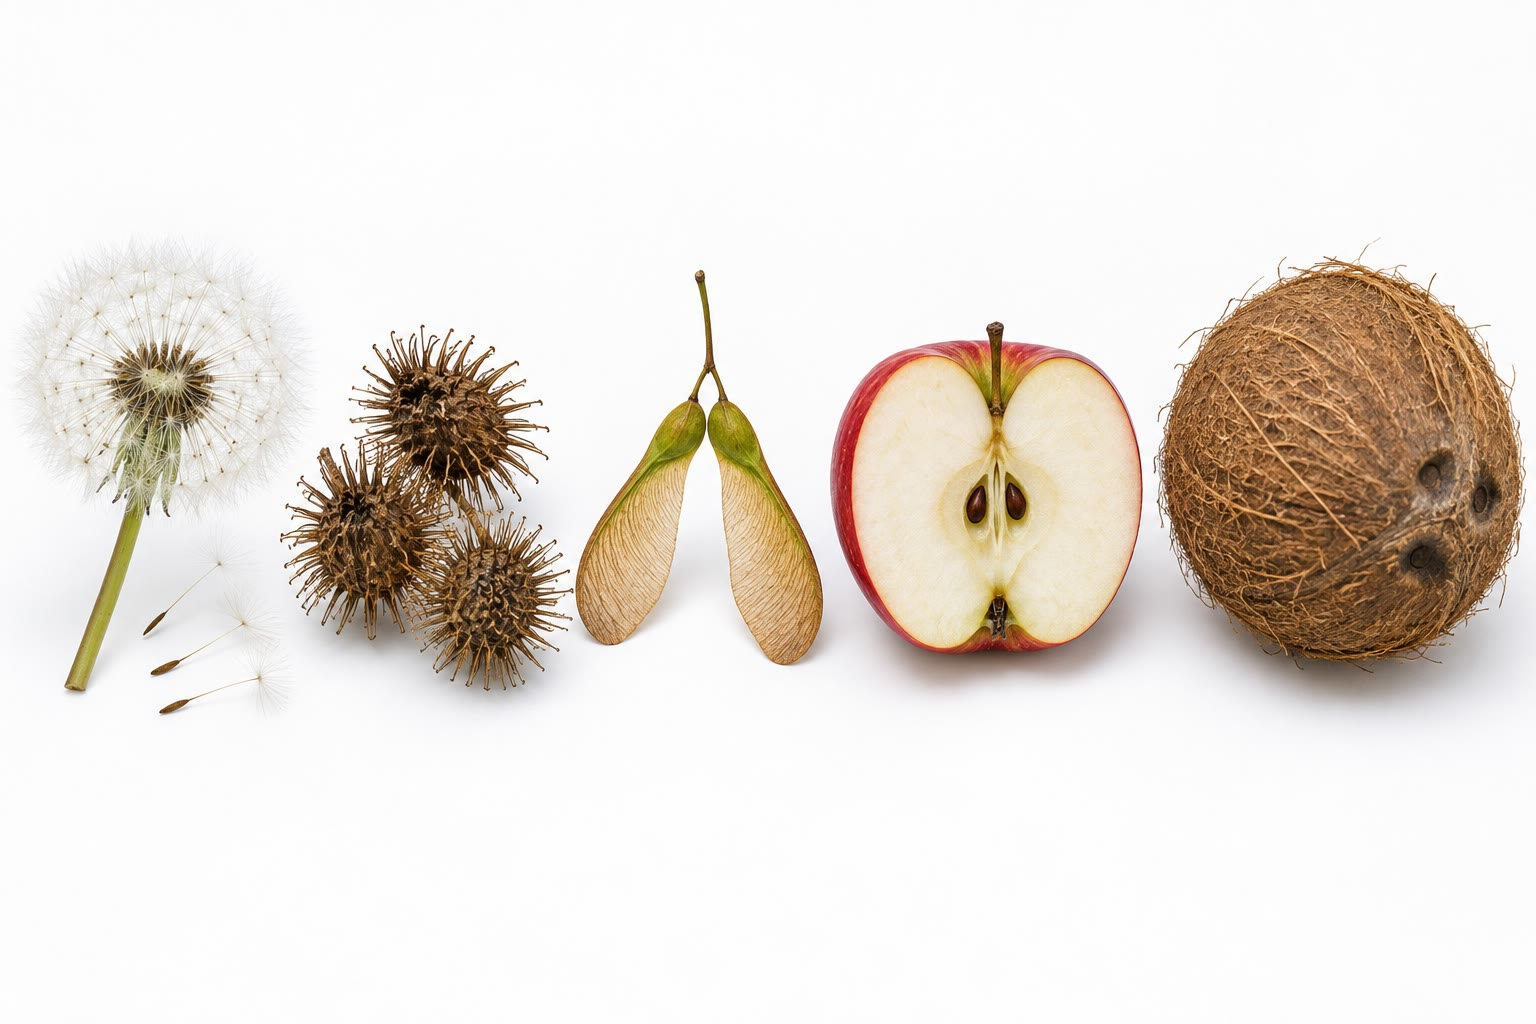
\includegraphics[width=0.62\linewidth]{images/book4/ai/b4-06-fruits-seeds.jpg}

{\small \omterm{def:b2:angiosperm-reproduction:seed}{Frutos} construidos para la dispersión: paracaídas (diente de
león), ganchos (bardana), alas (arce), carne para un animal (manzana) y
una cáscara flotante para el mar (coco).}
\end{omfigure}

\begin{example}[Distancias de dispersión]\label{ex:b2:angiosperm-reproduction:dispersal}
Un aquenio de diente de león con su vilano desciende a \qty{0.3}{m/s};
desde \qty{0.3}{m}, con un viento de \qty{3}{m/s}, vuela \qty{3}{m}, y
en una térmica, cientos. Una sámara de arce desciende girando sobre sí
misma a \qty{1}{m/s} desde \qty{15}{m}: \qty{45}{m}. Un hueso de cereza
que deja caer un ave tras veinte minutos de vuelo a \qty{10}{m/s}: hasta
\qty{12}{km}. Las bellotas de un roble caen a su pie, salvo que un
arrendajo se las lleve, cosa que hace por miles, a un kilómetro o más, y
olvida una décima parte: los robles que recolonizaron Europa tras la
última glaciación avanzaron hacia el norte a cientos de metros por año,
mucho más deprisa de lo que rueda una bellota, y fueron las aves las que
los desplazaron.
\end{example}

\section{Ejercicios}

\begin{exercise}[$\star$]\label{exo:b2:angiosperm-reproduction:1}
Nómbrense los cuatro verticilos de una \omterm{def:b2:angiosperm-reproduction:flower}{flor} y las partes de un \omterm{def:b2:angiosperm-reproduction:flower}{estambre}
y de un \omterm{def:b2:angiosperm-reproduction:flower}{carpelo}. ¿Qué partes son \omterm{def:b2:plant-life-cycles:cycles}{esporofito} \omterm{def:b2:meiosis-heredity:meiosis}{diploide} y cuáles
\omterm{def:b2:plant-life-cycles:cycles}{gametofito} \omterm{def:b2:meiosis-heredity:meiosis}{haploide}?
\end{exercise}

\begin{exercise}[$\star$]\label{exo:b2:angiosperm-reproduction:2}
Dese la ploidía de: una \omterm{def:b2:plant-life-cycles:heterospory}{microspora}, la célula vegetativa, una célula
espermática, la oosfera, un núcleo polar, el cigoto, el endospermo, la
\omterm{def:b2:angiosperm-reproduction:seed}{cubierta seminal}, la pared del \omterm{def:b2:angiosperm-reproduction:seed}{fruto}.
\end{exercise}

\begin{exercise}[$\star$]\label{exo:b2:angiosperm-reproduction:3}
Enumérense cinco rasgos de una \omterm{def:b2:angiosperm-reproduction:flower}{flor} anemófila y cinco de una \omterm{def:b2:angiosperm-reproduction:flower}{flor}
polinizada por abejas, y dese una planta de cada tipo.
\end{exercise}

\begin{exercise}[$\star$]\label{exo:b2:angiosperm-reproduction:4}
¿Qué es la \omterm{prop:b2:angiosperm-reproduction:double}{doble fecundación}, y qué produce cada una de las dos
fusiones? ¿Por qué puede decirse que el endospermo se fabrica ``por
encargo''?
\end{exercise}

\begin{exercise}[$\star\star$]\label{exo:b2:angiosperm-reproduction:5}
Una seda de maíz mide \qty{25}{cm} y un \omterm{thm:b2:angiosperm-reproduction:tube}{tubo polínico} crece a
\qty{1.2}{cm/h}. ¿Cuánto tarda la fecundación tras la \omterm{def:b2:angiosperm-reproduction:pollination}{polinización}? Una
panícula libera \omterm{def:b2:plant-life-cycles:heterospory}{polen} del día 0 al día 7 y las sedas de la planta
emergen del día 5 al día 12, una octava parte cada día; una seda solo
capta \omterm{def:b2:plant-life-cycles:heterospory}{polen} mientras se libera \omterm{def:b2:plant-life-cycles:heterospory}{polen}. ¿Qué fracción de las sedas queda
polinizada?
\end{exercise}

\begin{exercise}[$\star\star$]\label{exo:b2:angiosperm-reproduction:6}
Con autoincompatibilidad gametofítica, ¿qué fracción del \omterm{def:b2:plant-life-cycles:heterospory}{polen} es
compatible en los cruzamientos $S_1S_2\times S_1S_2$, $S_1S_2\times
S_1S_3$, $S_1S_2\times S_3S_4$ (primero el pistilo)? Dense los
\omterm{def:b2:meiosis-heredity:vocabulary}{genotipos} de los descendientes del segundo cruzamiento.
\end{exercise}

\begin{exercise}[$\star\star$]\label{exo:b2:angiosperm-reproduction:7}
En una población con $n$ \omterm{def:b2:meiosis-heredity:vocabulary}{alelos} $S$ igual de frecuentes, ¿qué fracción
del \omterm{def:b2:plant-life-cycles:heterospory}{polen} tomado al azar es compatible con una planta dada? Explíquese
por qué se propaga un nuevo \omterm{def:b2:meiosis-heredity:vocabulary}{alelo} $S$ surgido por \omterm{def:b2:genome-diversification:mutation}{mutación}, y qué predice
esto sobre el número de \omterm{def:b2:meiosis-heredity:vocabulary}{alelos}.
\end{exercise}

\begin{exercise}[$\star\star$]\label{exo:b2:angiosperm-reproduction:8}
Una planta de maíz heterocigota $Yy$ (endospermo amarillo \omterm{def:b2:meiosis-heredity:vocabulary}{dominante}) se
autofecunda. Dense los \omterm{def:b2:meiosis-heredity:vocabulary}{genotipos} del endospermo de sus granos y sus
proporciones, recordando que los dos \omterm{prop:b2:angiosperm-reproduction:embryosac}{núcleos polares} son idénticos. ¿Qué
fracción de los granos es amarilla? ¿Y si la planta es polinizada por una
planta $yy$?
\end{exercise}

\begin{exercise}[$\star\star$]\label{exo:b2:angiosperm-reproduction:9}
Descríbase el experimento de la aleurona y explíquese qué muestra sobre
(a) el papel del embrión, (b) el papel de la giberelina, (c) el lugar de
síntesis de la amilasa. ¿Por qué el medio grano sin embrión es el
control esencial?
\end{exercise}

\begin{exercise}[$\star\star\star$]\label{exo:b2:angiosperm-reproduction:10}
Compárense en coste las estrategias anemófila y zoófila: una planta
anemófila fabrica $10^{6}$ granos por óvulo a \qty{1}{\micro g} cada uno;
una planta zoófila fabrica $10^{3}$ granos por óvulo a \qty{1}{\micro g}
cada uno, más \qty{5}{mg} de azúcar de \omterm{def:b2:angiosperm-reproduction:pollination}{néctar} por \omterm{def:b2:angiosperm-reproduction:flower}{flor} de diez óvulos.
Calcúlese el coste reproductivo por óvulo en cada caso (tómense el \omterm{def:b2:plant-life-cycles:heterospory}{polen}
y el azúcar con la misma energía por gramo), y explíquese por qué la
\omterm{def:b2:angiosperm-reproduction:pollination}{polinización} por el viento persiste pese a todo.
\end{exercise}

\begin{exercise}[$\star\star\star$]\label{exo:b2:angiosperm-reproduction:11}
Explíquese, con las cifras del \cref{ex:b2:angiosperm-reproduction:dispersal},
por qué un \omterm{def:b2:angiosperm-reproduction:seed}{fruto} carnoso compensa su coste a un árbol aunque el animal
digiera la pulpa y deje caer la mayoría de las \omterm{def:b2:angiosperm-reproduction:seed}{semillas} donde no pueden
crecer.
\end{exercise}

\begin{exercise}[$\star\star\star$]\label{exo:b2:angiosperm-reproduction:12}
``El \omterm{def:b2:angiosperm-reproduction:flower}{carpelo} cerrado es la razón por la que las plantas con \omterm{def:b2:angiosperm-reproduction:flower}{flores}
dominan la tierra firme.'' Discútase: qué hace posible el encierro del
óvulo (elección del \omterm{def:b2:plant-life-cycles:heterospory}{polen}, incompatibilidad, el \omterm{def:b2:angiosperm-reproduction:seed}{fruto}) y qué cuesta.
\end{exercise}

\section{Problema: un huerto y un campo}

\begin{problem}[{Problema de fin de semana --- la polinización de un
manzanar planificada en torno a la autoincompatibilidad, y la fecundación
y el rendimiento de un campo de maíz calculados a partir del polen que
produce, hasta llegar al cuajado del huerto y al número de granos del
campo}]
\label{pb:b2:angiosperm-reproduction:1}
El manzano es gametofíticamente autoincompatible. Un huerto tiene tres
variedades: A ($S_1S_2$), B ($S_1S_3$), C ($S_3S_4$). Una \omterm{def:b2:angiosperm-reproduction:flower}{flor} tiene
cinco \omterm{def:b2:angiosperm-reproduction:flower}{carpelos} con dos óvulos cada uno, y el árbol deja caer todo \omterm{def:b2:angiosperm-reproduction:seed}{fruto}
que forme menos de cinco \omterm{def:b2:angiosperm-reproduction:seed}{semillas}. Una visita de abeja deposita
\num{100} \omterm{prop:b2:angiosperm-reproduction:pollen}{granos de polen} en un \omterm{def:b2:angiosperm-reproduction:flower}{estigma}; cada grano compatible tiene una
probabilidad de $0.1$ de fecundar un óvulo aún libre. Un árbol lleva
\num{5000} \omterm{def:b2:angiosperm-reproduction:flower}{flores} y necesita \num{250} \omterm{def:b2:angiosperm-reproduction:seed}{frutos} para una cosecha completa.
Maíz: una panícula libera
$10^{7}$ granos a lo largo de \num{7} días; el campo tiene \num{8}
plantas por metro cuadrado; cada planta lleva una mazorca de \num{600}
sedas; una seda
presenta \qty{1e-4}{m^2} al \omterm{def:b2:plant-life-cycles:heterospory}{polen} que cae; el \omterm{def:b2:plant-life-cycles:heterospory}{polen} se deposita a
\qty{0.25}{m/s}; un grano de maíz contiene \qty{0.3}{g} de endospermo.

\medskip
\noindent\textbf{Parte I --- Compatibilidad.}
\begin{enumerate}
  \item Para el \omterm{def:b2:plant-life-cycles:heterospory}{polen} de cada variedad sobre un pistilo de A, dese la
        fracción compatible $f$.
  \item Lo mismo para pistilos de B y de C.
  \item Una abeja que llega de un árbol de B deposita 100 granos en un
        \omterm{def:b2:angiosperm-reproduction:flower}{estigma} de A: ¿cuántos son compatibles, y cuántos óvulos cabe
        esperar que se fecunden (despréciese la saturación)?
  \item Lo mismo para una abeja que viene de C, y de otro A.
  \item ¿Qué \omterm{def:b2:angiosperm-reproduction:seed}{frutos} se conservan? ¿Qué riesgo tiene plantar un huerto
        solo de la variedad A?
  \item Un bloque de árboles A está rodeado de árboles C; la mitad de las
        visitas de abeja a A proceden de C. Si cada \omterm{def:b2:angiosperm-reproduction:flower}{flor} recibe una
        visita, ¿qué fracción de las \omterm{def:b2:angiosperm-reproduction:flower}{flores} de A cuaja \omterm{def:b2:angiosperm-reproduction:seed}{fruto}, y cuántos
        \omterm{def:b2:angiosperm-reproduction:seed}{frutos} da cada árbol? ¿Es completa la cosecha?
  \item ¿Por qué se intercala en los huertos un manzano silvestre que
        florece durante semanas, y por qué hay que comprobar sus \omterm{def:b2:meiosis-heredity:vocabulary}{alelos}
        $S$?
\end{enumerate}

\medskip
\noindent\textbf{Parte II --- El \omterm{def:b2:plant-life-cycles:heterospory}{polen} sobre el campo de maíz.}
\begin{enumerate}[resume]
  \item Calcúlese el \omterm{def:b2:plant-life-cycles:heterospory}{polen} liberado por metro cuadrado de campo y por
        segundo, en promedio a lo largo de los siete días.
  \item En estado estacionario, el flujo de \omterm{def:b2:plant-life-cycles:heterospory}{polen} que se deposita es igual
        a la tasa de liberación. Calcúlese la concentración de \omterm{def:b2:plant-life-cycles:heterospory}{polen} en
        el aire (granos por metro cúbico).
  \item Calcúlense el número de granos que caen sobre una seda por
        segundo y el tiempo medio de espera hasta el primer grano.
  \item ¿Cuántos granos recibe una seda en un día? ¿Por qué solo es útil
        el primero?
  \item Se poliniza una seda de \qty{20}{cm}; el tubo crece a
        \qty{1}{cm/h}. ¿Cuándo se fecunda el óvulo?
  \item Una sequía retrasa cinco días la emergencia de las sedas mientras
        la panícula libera el \omterm{def:b2:plant-life-cycles:heterospory}{polen} según lo previsto. Con el periodo de
        liberación de siete días, estímense la fracción de la temporada de
        \omterm{def:b2:plant-life-cycles:heterospory}{polen} que captan las sedas y la consecuencia para el rendimiento.
\end{enumerate}

\medskip
\noindent\textbf{Parte III --- La \omterm{prop:b2:angiosperm-reproduction:double}{doble fecundación} y el grano.}
El campo es de una variedad de endospermo amarillo ($Y$, \omterm{def:b2:meiosis-heredity:vocabulary}{dominante}) y
linda con un campo blanco ($yy$); el viento sopla desde el campo blanco.
\begin{enumerate}[resume]
  \item Dense los \omterm{def:b2:meiosis-heredity:vocabulary}{genotipos} del embrión y del endospermo de un grano de
        una planta $YY$ fecundada por \omterm{def:b2:plant-life-cycles:heterospory}{polen} $yy$.
  \item ¿Es el grano amarillo o blanco? Explíquese el término xenia.
  \item Una planta $Yy$ es polinizada por \omterm{def:b2:plant-life-cycles:heterospory}{polen} $yy$: dense los
        \omterm{def:b2:meiosis-heredity:vocabulary}{genotipos} del endospermo y sus frecuencias.
  \item El endospermo contiene dos genomas maternos y uno paterno. Un gen
        con efecto de dosis da, por copia, 10~unidades de pigmento: ¿qué
        cantidad de pigmento llevan los granos $YYy$, $Yyy$ e $yyY$ (dos
        dosis paternas, hipotéticamente)? ¿Cuáles de ellos pueden existir
        realmente?
  \item Explíquese por qué lo que comemos es el endospermo y no el
        embrión, y qué fracción de la masa del grano representa si el
        embrión pesa \qty{0.03}{g}.
  \item ¿Por qué el aprovisionamiento ``por encargo'' del endospermo es
        una ventaja frente al de las gimnospermas?
\end{enumerate}

\medskip
\noindent\textbf{Parte IV --- Rendimiento.}
\begin{enumerate}[resume]
  \item Si se fecunda el \qty{90}{\%} de las sedas, calcúlense los granos
        por mazorca, por planta y por metro cuadrado, y la masa de
        endospermo por metro cuadrado.
  \item Conviértase en toneladas por hectárea.
  \item El cultivo fija \qty{1.2}{kg} de carbono por metro cuadrado por
        temporada, de los cuales la mitad acaba en el grano cosechado.
        Compruébese la coherencia con la masa de la pregunta 20 (el
        endospermo contiene un \qty{45}{\%} de carbono).
  \item ¿Cuántos \omterm{prop:b2:angiosperm-reproduction:pollen}{granos de polen} liberó el campo por grano cosechado?
  \item Explíquese por qué una planta de maíz aislada en un jardín forma
        una mazorca mal granada.
  \item Enúnciese el resultado: el cuajado del bloque A y el rendimiento
        del campo en granos por metro cuadrado y en toneladas por
        hectárea.
\end{enumerate}
\end{problem}
